%\right \right \right \right \right \right \right \right \right \right \right \right \right \right \right \right \right \right \right \right \right \right \right \right \right \right \right \right \right \right \right \right \right \right \right \right \right \right \right \right \right \right \right \right \right \right \right \right \right 	~~~~~~~~```% This is "sig-alternate.tex" V2.0 May 2012
% This file should be compiled with V2.5 of "sig-alternate.cls" May 2012
%
% This example file demonstrates the use of the 'sig-alternate.cls'
% V2.5 LaTeX2e document class file. It is for those submitting
% articles to ACM Conference Proceedings WHO DO NOT WISH TO
% STRICTLY ADHERE TO THE SIGS (PUBS-BOARD-ENDORSED) STYLE.
% The 'sig-alternate.cls' file will produce a similar-looking,
% albeit, 'tighter' paper resulting in, invariably, fewer pages.
%
% ----------------------------------------------------------------------------------------------------------------
% This .tex file (and associated .cls V2.5) produces:
%       1) The Permission Statement
%       2) The Conference (location) Info information
%       3) The Copyright Line with ACM data
%       4) NO page numbers
%
% as against the acm_proc_article-sp.cls file which
% DOES NOT produce 1) thru' 3) above.
%
% Using 'sig-alternate.cls' you have control, however, from within
% the source .tex file, over both the CopyrightYear
% (defaulted to 200X) and the ACM Copyright Data
% (defaulted to X-XXXXX-XX-X/XX/XX).
% e.g.
% \CopyrightYear{2007} will cause 2007 to appear in the copyright line.
% \crdata{0-12345-67-8/90/12} will cause 0-12345-67-8/90/12 to appear in the copyright line.
%
% ---------------------------------------------------------------------------------------------------------------
% This .tex source is an example which *does* use
% the .bib file (from which the .bbl file % is produced).
% REMEMBER HOWEVER: After having produced the .bbl file,
% and prior to final submission, you *NEED* to 'insert'
% your .bbl file into your source .tex file so as to provide
% ONE 'self-contained' source file.
%
% ================= IF YOU HAVE QUESTIONS =======================
% Questions regarding the SIGS styles, SIGS policies and
% procedures, Conferences etc. should be sent to
% Adrienne Griscti (griscti@acm.org)
%
% Technical questions _only_ to
% Gerald Murray (murray@hq.acm.org)
% ===============================================================
%
% For tracking purposes - this is V2.0 - May 2012

\documentclass{sig-alternate}
\usepackage[normalem]{ulem}
\usepackage{algpseudocode}
\usepackage{algorithm}
\usepackage{amsmath}
%\usepackage{url}
\usepackage{graphicx}
\usepackage{subfigure}

\usepackage{footnote}
\makesavenoteenv{tabular}
\makesavenoteenv{table}

\algrenewcommand{\algorithmicrequire}{\textbf{Input:}}
\algrenewcommand{\algorithmicensure}{\textbf{Output:}}
\renewcommand{\algorithmicforall}{\textbf{for each}}

\begin{document}
%
% --- Author Metadata here ---
\conferenceinfo{WOODSTOCK}{'97 El Paso, Texas USA}
%\CopyrightYear{2007} % Allows default copyright year (20XX) to be over-ridden - IF NEED BE.
%\crdata{0-12345-67-8/90/01}  % Allows default copyright data (0-89791-88-6/97/05) to be over-ridden - IF NEED BE.
% --- End of Author Metadata ---

\title{Error Locating Driven Array\titlenote{This work was supported by the National Natural Science Foundation of China (No. 61272079), the Research Fund for the Doctoral Program of Higher Education of China (No.20130091110032), the Science Fund for Creative Research Groups of the National Natural Science Foundation of China(No. 61321491), and the Major Program of National Natural Science Foundation of China (No. 91318301)}
}
%
% You need the command \numberofauthors to handle the 'placement
% and alignment' of the authors beneath the title.
%
% For aesthetic reasons, we recommend 'three authors at a time'
% i.e. three 'name/affiliation blocks' be placed beneath the title.
%
% NOTE: You are NOT restricted in how many 'rows' of
% "name/affiliations" may appear. We just ask that you restrict
% the number of 'columns' to three.
%
% Because of the available 'opening page real-estate'
% we ask you to refrain from putting more than six authors
% (two rows with three columns) beneath the article title.
% More than six makes the first-page appear very cluttered indeed.
%
% Use the \alignauthor commands to handle the names
% and affiliations for an 'aesthetic maximum' of six authors.
% Add names, affiliations, addresses for
% the seventh etc. author(s) as the argument for the
% \additionalauthors command.
% These 'additional authors' will be output/set for you
% without further effort on your part as the last section in
% the body of your article BEFORE References or any Appendices.

\numberofauthors{3} %  in this sample file, there are a *total*
% of EIGHT authors. SIX appear on the 'first-page' (for formatting
% reasons) and the remaining two appear in the \additionalauthors section.
%
\author{
% You can go ahead and credit any number of authors here,
% e.g. one 'row of three' or two rows (consisting of one row of three
% and a second row of one, two or three).
%
% The command \alignauthor (no curly braces needed) should
% precede each author name, affiliation/snail-mail address and
% e-mail address. Additionally, tag each line of
% affiliation/address with \affaddr, and tag the
% e-mail address with \email.
%
% 1st. author
\alignauthor
Xintao Niu\\
       \affaddr{State Key Laboratory for Novel Software Technology}\\
       \affaddr{Nanjing University}\\
       \affaddr{China, 210023}\\
       \email{niuxintao@gmail.com}
% 2nd. author
\alignauthor
Changhai Nie\\
       \affaddr{State Key Laboratory for Novel Software Technology}\\
       \affaddr{Nanjing University}\\
       \affaddr{China, 210023}\\
       \email{changhainie@nju.edu.cn}
% 3rd. author'
\alignauthor
JiaXi Xu\\
       \affaddr{School of Mathematics and Information Technology}\\
       \affaddr{Nanjing Xiaozhuang University}\\
       \affaddr{China, 211171}\\
       \email{xujiaxi@126.com}
}
% There's nothing stopping you putting the seventh, eighth, etc.
% author on the opening page (as the 'third row') but we ask,
% for aesthetic reasons that you place these 'additional authors'
% in the \additional authors block, viz.
% Just remember to make sure that the TOTAL number of authors
% is the number that will appear on the first page PLUS the
% number that will appear in the \additionalauthors section.
\maketitle
\begin{abstract}
Combinatorial testing(CT) seeks to handle potential faults caused by various interactions of factors that can influence the Software systems. When applying CT, it is a common practice to first generate a bunch of test cases to cover each possible interaction and then to locate the failure-inducing interaction if any failure is detected. Although this conventional procedure is simple and straightforward, we conjecture that it is not the ideal choice in practice. This is because 1) testers desires to isolate the root cause of failures before all the needed test cases are generated and executed 2) the early located failure-inducing interactions can guide the remaining test cases generation, such that many unnecessary and invalidate test cases can be avoided. For this, we propose a novel CT framework that allows for both generation and localization process to better share each other's information, as a result, both this two testing stages will be more effectively and efficiently when handling the testing tasks. We conducted a series of empirical studies on several open-source software, of which the result shows that our framework can locate the failure-inducing interactions more quickly than traditional approaches, while just needing less test cases.
%When the system under test(SUT) is suffered from interations faults such as option compliant, testers want to design. As . Efficenet test space is desired when . To handle this problem, the art of  is to design a t-way covering array, which can cover all the t-way , just using small size of test cases. In this paper, however, we conjecture that the covering array is somewhat reduntant with respect to fault locating. The main reason for the reduntance the we find is the framework it takes is not efficent, traditional works will first generate a covering array to detect if any failing is triggered by any test case, and then pick these failing test case to further locating. In CT, most locating teachinques is just to generate addtional test cases to isolate the MFS. We find two shortcoming for this framework 1: if we had first identify some MFS, we do not need to generate any test case to conatin them, further, any combination contain this MFS will not need to be covered, 2: if we do not genrate, the extra test cases will support some coverage is that when we first already covered. So for this two points, in this paper, we propose a new framework to make the generating process and isolating process more tightly so that the isolating process and generating process will better utilize each other. We have done some emprical studies on several open-source software and found that our new frame work can significantly reduce the test cases.
%Combinatorial testing(CT) is proven to be effective to reveal the potential failures caused by the interaction of the inputs or options of the System Under Test(SUT). A key problem in CT is to isolate the failure-inducing combinations of the related failure as it can facilitate the debugging efforts by reducing the scope of code that needs to be inspected. Many algorithms has been proposed to identify such combinations, however, most of these studies either just consider the condition of one fault or ignore masking effects among multiple faults which can bias their identified results. In this paper, we analysed how the masking effect of multiple faults affect on the isolation of failure-inducing combinations. We further give a strategy of selecting test cases to alleviate this impact, which works by pruning these test cases that may trigger masking effect and replacing them with no-masking-effect ones. The test case selecting process repeated until we get enough information to isolate the failure-inducing combinations. We conducted some empirical studies on several open-source software. The result of the studies shows that multiple faults as well as the masking effects do exist in real software and our approach can assist combinatorial-based failure-inducing identifying methods to get a better result when handling multiple faults in SUT.
\end{abstract}

% A category with the (minimum) three required fields
%\category{H.4}{Information Systems Applications}{Miscellaneous}
%A category including the fourth, optional field follows...
\category{D.2.5}{Software Engineering}{Testing and debugging}[Debugging aids,testing tools]

\terms{Reliability, Verification}

\keywords{Software Testing, Combinatorial Testing, Covering Array, Failure-inducing combinations} % NOT required for Proceedings

\section{Introduction}

Modern software is developed more sophisticatedly and intelligently than before. To test such software is challenging, as the candidate factors that can influence the system's behaviour, e.g., configuration options, system inputs, message events, are enormous. Even worse, the interactions between these factors can also crash the system, e.g., the compatibility problems. In consideration of the scale of the real industrial software, to test all the possible combination of all the factors (we call them the interaction space) is not feasible, and even it is possible, it is not recommended to test exhaustive interactions for most of them do not provide any useful information.

Many empirical studies shows that in real software systems, the effective interaction space, i.e., targeting fault defects, makes up only a small proportion of the overall interaction space. What's more, the number of factors involved in these effective interactions is relatively small, of which 4-6 is usually the upper bonds. With this observation, applying CT in practice is appealing, as it is proven to be effective to handle the interaction faults in the system.

A typical CT life-circle is listed as Figure \ref{ct-life}, in which there are four main testing stages. At the very beginning of the testing, engineers should extract the specific model of the software under test. In detail, they should identify the factors, such as user inputs, configure options, environment states and the like that could affect the system's behavior. Next, which values each factor can take should also be determined. Further efforts will be needed to figure out the constraints and dependencies between each factor and corresponding values to make the testing work valid. After the modeling stage, a bunch of test cases should be generated and executed to expose the potential faults in the system. In CT, one test case is a set of assignment of all the factors that we modeled before. Thus, when such a test case is executed, all the interactions contained in the test case are deemed to be checked. The main target of this stage is to design a relatively small size of test cases to get some specific coverage, for CT the most common coverage is to check all the possible interactions with the number of factors no more than a prior fixed integer, i.e., strength \emph{t}. The third testing stage in this circle is the fault localization, which is responsible for diagnosing the root cause of the failure we detected before. To characterize such root cause, i.e., failure-inducing interactions of corresponding factors and values is important for future bug fixing, as it will reduce the suspicious code scope that needed to inspect. The last testing stage of CT is evaluation. In this stage, testers will assess the quality of the previously conducted testing tasks, many metrics such as whether the failure-inducing interactions can reflect the failures detected, whether the generated test cases is adequate to expose all the behaviors of the system,  will be validated. And if the assessment result shows that the previous testing process does not fulfil the testing requirement, some testing stages should be made some improvement, and sometimes, may even need to be re-conducted.

Although this conventional CT framework is simple and straightforward, however in terms of the test cases generation and fault localization stages, we conjecture that the first-generation-then-localization is not the proper choice for most test engineers. This is because, first, it is not realistic for testers wait for all the needed test cases are generated before they can diagnosis and fix the failures that haven been detected, second, and the most important, utilizing the early determined failure-inducing interactions can guide the following test cases generations, such that many unnecessary and invalid test cases will be avoided. For this we get to the most key idea of this paper:

\emph{Generation and Localization process should be organised in a more tightly way.}

Based on the idea, we propose a new CT framework, which instead of dividing the generation and localization into two independent stages, it integrate this two stages into one. We call this new one the Generation-Localization stage, which allows for both generation and localization better share each other's testing information. To this aim, we remodel the generation and localization modular to make them better adapt to this newly framework. In specific, our generation adopts the one-test-one-time strategy, i.e., generate and execute one test case in one iteration. Rather than generating the overall needed test cases in one time, this strategy is more flexible so that it allows for terminating at any time during generation, no matter whether the coverage is reached or not. With this strategy, we can let the generation stops at the point we detect some failures, and then after localization we can utilize the diagnosing result to change the coverage criteria, e.g., the interactions related to the failure-inducing interactions do not need to be checked any more. Then based on the new coverage criteria, the generation process goes on.

%For the fault localization, we augment this process with a test case . instead of independently generating extra test cases, we add a new process to let it can get a guide . we will also take use of the test cases generation before, this will shows in the extra test case. Fault localization will need more.

We conducted a series empirical studies on several open-source software to evaluate our newly framework. In short, we take two main comparisons, one is to compare our new framework with the traditional one, which first generate a complete set of test cases and then perform the fault localization. Another one is to compare with the Error locating array, which is a well-designed set of test cases that can be used directly detect and isolate the failure-inducing interactions. The results shows that in terms of test case generation and fault diagnosis, our approach can and significantly reduced the overall needed test cases and can more quickly isolate the root cause of the system under test.

The main contributions of this paper:

 \begin{enumerate}
 \item  We propose a newly CT framework which combine the test cases generation and fault localization more closely.
 \item  We augment the traditional CT test cases generation and fault localization process to make them adapt to the newly framework.
 \item  A series comparisons with traditional CT is conducted and the result of the empirical studies are discussed.
\end{enumerate}


The reset of the paper is organised as follows: Section 2 presents the preliminary background of some definitions of the CT.  Section 3 describes our newly framework and a simple case study is also given. Section 4 presents the empirical studies and the results are discussed. Section 5 shows the related works. Section 6 concludes the paper and propose some further works.


% Cohen[] studies the , and find 70 ~ 100 can be. []Shows that to get a some coverage, only a small subset of all the configuration is needed. To this aim,
%
%Typically, when applying CT in practice, there are four testing stages that should be cated as in figure. At the very early of the testing work, engineers should characterize which options and what inputs , i.e., to identify the factors and their possible values. This stage is labor-consuming, at least in the initial testing. The second stage is to generate a bunch of test cases to meet some criteria. In CT, the most common scenario is to cover all the iterations with the factors in the interactions no more than a prior fixed number -- t, in such way, the test suites of CT is also called the t-way covering array.  The third testing stage is to fault localization, i.e., to isolate the failure-inducing interactions which owes to those failures triggered in those test cases in these test cases. The final stage is to evaluate the quality of the test cases.
%
%This conventional CT framework is simple and straight forward, however, we conjecture, it is not he suiable choices and not the choices for most test engineers.  The first,   Second, and most importantly, is.
%
%For this, we.


\begin{figure}
 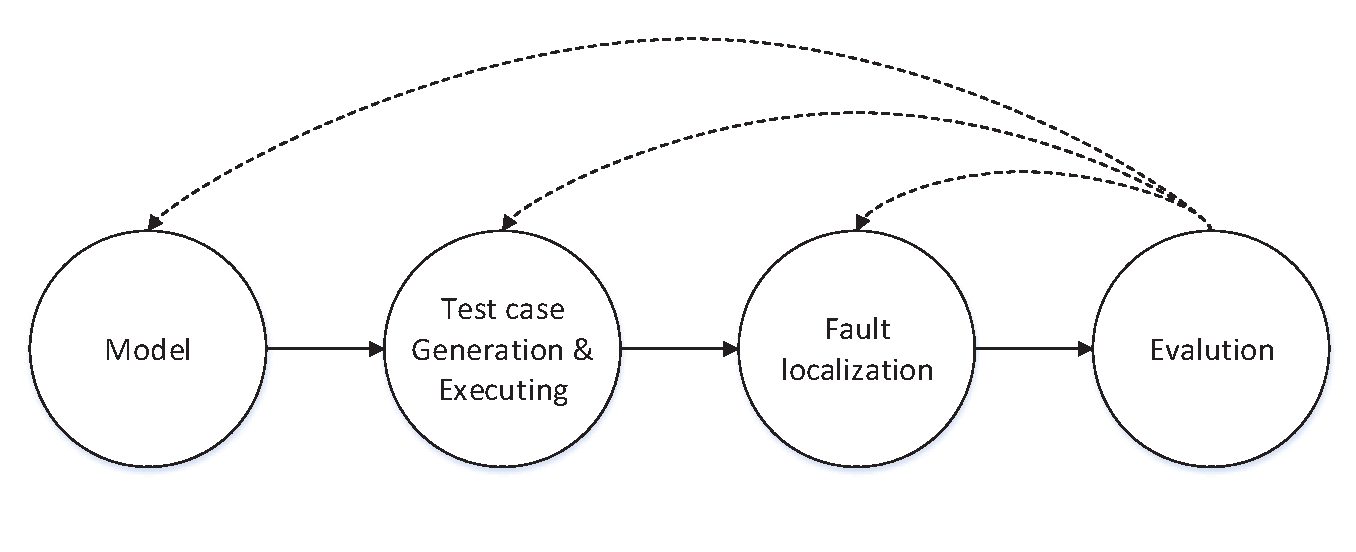
\includegraphics[width=3.4in]{CT_lifecircle.eps}
\caption{The life circle of CT}
\label{ct-life}
\end{figure}
%Software system are growing more and more complexity, the testing is needed. Nowadays, the bugs are not the single factor-bug, that is, it is . To detect and isolate such a is hard, for we could not easily know which interaction of from so many. The first, how to detect, the second, even if we have detected, .


%
%Combinatorial testing is a proposing testing technique to handle such problem. The testing object-- covering array is a well designed test suite, which can cover each possible interaction with just a small or reasonable size. When one or more test cases trigger some fault, it take the isolating.asdlajsdlas-d=
%
%In CT it is a pri-critira that the test suite must be , and then using to trigger. This framework is straight and simple, however, we conjecture in this paper that this would be more redundant inspect of fault debugging. Through a series experiment on empirical study, we observe that, there is two main : right . wrong .   This redundant can make the tester to test more unnecessary test cases, which is a wasting of computing resource.
%
%So in this paper, we propose a new and really intuial CT fault detecting and isolating framework (CTDI), which combine the more tightly. In detail our framework, handles two main . For we find . we make it as constraint, and feedback to the generating. The second, as we can generate many extra test cases, for these passing test cases, we use them as seed to let them in the generating process. The ended criteria is some coverage is reached.
%
%Our new CT is .
%
%We have imply , and find our approach can .



%
%With the increasing complexity and size of modern software, many factors, such as input parameters and configuration options, can influence the behaviour of the SUT. The unexpected faults caused by the interaction among these factors can make testing such software a big challenge if the interaction space is too large. One remedy for this problem is combinatorial testing, which systematically sample the interaction space and select a relatively small set of test cases that cover all the valid iterations with the number of factors involved in the interaction no more than a prior fixed integer, i.e., the \emph{strength} of the interaction.
%
%Once failures are detected, it is desired to isolate the failure-inducing combinations in these failing test cases. This task is important in CT as it can facilitate the debugging efforts by reducing the code scope that needed to inspected.

%\section{Motivating example}
%Combinatorial testing can effectively detect the failures caused by the interactions between various options or inputs of the SUT. Covering arrays, the test suite generated by this technique can cover each combination of the options at least once. We conjecture, however, although covering array can effectively, in practice, covering array was too much for detecting and locating the error in particular software.
%
%As an motivating example, we looked through the following scenarios for detecting and locating the errors in the SUT.
%
%Too much redundant fault test cases:
%
%
%Too much redundant right test cases:

\section{Background}
This section presents some definitions and propositions to give a formal model for the FCI problem.

\subsection{Failure-inducing combinations in CT}

Assume that the SUT is influenced by \emph{n} parameters, and each parameter $p_{i}$ has $a_{i}$ discrete values from the finite set $V_{i}$, i.e., $a_{i}$ = $|V_{i}|$ ($i$ = 1,2,..n). Some of the definitions below are originally defined in .

\newdef{definition}{Definition}
\begin{definition}
A \emph{test case} of the SUT is an array of \emph{n} values, one for each parameter of the SUT, which is denoted as a \emph{n}-tuple ($v_{1}$, $v_{2}$,...,$v_{n}$), where $v_{1}\in V_{1}$, $v_{2} \in V_{2}$ ... $v_{n} \in V_{n}$.
\end{definition}

In practice, these parameters in the test case can represent many factors, such as input variables, run-time options, building options or various combination of them. We need to execute the SUT with these test cases to ensure the correctness of the behaviour of the software.

%\begin{definition}
We consider the fact that the abnormally executing test cases as a \emph{fault}. It can be a thrown exception, compilation error, assertion failure or constraint violation. When faults are triggered by some test cases, what is desired is to figure out the cause of these faults, and hence some subsets of this test case should be analysed.
%\end{definition}

%Figuring out the test case as well as the executing result is usually not enough to analyse the source of the bug, especially when there are too many parameters we need to care in this test case. In this circumstance, we need to study some subsets of this test case, so we need the following definition:

%Figuring out the execution outcomes of test cases must reveal the presence of faulty interactions among those considered. However, the location and magnitude of the fault is still far from clear, especially when there are too many parameters we need to care in this test case. Hence, we need to study some subsets of this test case, which can help isolate the cause of failures.

\begin{definition}
For the SUT, the \emph{n}-tuple (-,$v_{n_{1}}$,...,$v_{n_{k}}$,...)is called a \emph{k}-value \emph{combination} ($0 < k \leq n $) when some k parameters have fixed values and the others can take on their respective allowable values, represented as ``-".

In effect a test case itself is a k-value \emph{combination}, when k = n. Furthermore, if a test case contain a \emph{combination}, i.e., every fixed value in the combination is in this test case, we say this test case \emph{hits} the \emph{combination}.
%, which can be denoted as $k-value\  combination \in T$
\end{definition}

\begin{definition}
let $c_{l}$ be a \emph{l}-value combination, $c_{m}$ be an \emph{m}-value combination in SUT and $l < m$. If all the fixed parameter values in $c_{l}$ are also in $c_{m}$, then $c_{m}$ \emph{subsumes} $c_{l}$. In this case we can also say that $c_{l}$ is a \emph{sub-combination} of $c_{m}$ and $c_{m}$ is a \emph{parent-combination} of $c_{l}$, which can be denoted as $c_{l} \prec  c_{m}$.
\end{definition}

For example, in the motivation example section, the 2-value combination (-, 4, 4, -) is a sub-combination of the 3-value combination (-, 4, 4, 5), that is, (-,4,4,-) $\prec$ (-,4,4,5).

\begin{definition}
If all test cases contain a combination, say $c$, trigger a particular fault, say $F$, then we call this combination $c$ the \emph{faulty combination} for $F$. Additionally, if none sub-combination of $c$ is the \emph{faulty combination} for $F$, we then call the combination $c$ the \emph{minimal faulty combination} for $F$ (It is also called Minimal failure-causing schema(MFS) in ).

%Based on this, if a test case $t$ hit such a failure-inducing combination, say $c(F)$, it should trigger the fault $F$, for which the test case can be put as $t(F)$
\end{definition}

In fact, MFS and \emph{minimal faulty combinations} are identical to the failure-inducing combinations we discussed previously. Figuring it out can eliminate all details that are irrelevant for causing the failure and hence facilitate the debugging efforts.

\section{Algorithms}

\subsection{Description}

\subsection{A case study}

\section{empirical studies}


\subsection{The existence of }


\subsubsection{Study setup}


\subsubsection{Result and discusssion}


\subsection{Performance of the traditional algorithms}

\subsubsection{Study setup}

\subsubsection{Result and discussion}


\subsection{Performance of our approach}

%, and then we applied these augmented approaches to identify the failure-inducing combinations in the prepared subjects.

\subsubsection{Study setup}


%Additionally, comparisons between the augmented approaches and three traditional ones will be quantified.

\subsubsection{Result and discussion}


\subsection{Threats to validity}


\section{related works}


\section{Conclusions}


%\end{document}  % This is where a 'short' article might terminate

%ACKNOWLEDGMENTS are optional
%\section{Acknowledgments}
%This section is optional; it is a location for you
%to acknowledge grants, funding, editing assistance and
%what have you.  In the present case, for example, the
%authors would like to thank Gerald Murray of ACM for
%his help in codifying this \textit{Author's Guide}
%and the \textbf{.cls} and \textbf{.tex} files that it describes.

%
% The following two commands are all you need in the
% initial runs of your .tex file to
% produce the bibliography for the citations in your paper.
\bibliographystyle{abbrv}
%\bibliographystyle{unsrt}
\bibliography{sigproc}  % sigproc.bib is the name of the Bibliography in this case
% You must have a proper ".bib" file
%  and remember to run:
% latex bibtex latex latex
% to resolve all references
%
% ACM needs 'a single self-contained file'!
%
%APPENDICES are optional
%\balancecolumns
%\appendix
%%Appendix A
\end{document}
